\documentclass[12pt, twoside]{article}
\usepackage{jmlda}
\newcommand{\hdir}{.}

\renewcommand{\baselinestretch} {1.35}

\usepackage{graphicx}
\usepackage{caption}
\usepackage{subfig}
\graphicspath{{phase/}}
\DeclareGraphicsExtensions{.pdf,.png,.jpg}

\begin{document}

\title
    [] % краткое название; не нужно, если полное название влезает в~колонтитул
    {Определение фазы и разладки движения человека по сигналам носимых устройств}
\author
    [А.\,Д.~Курдюкова] % список авторов (не более трех) для колонтитула; не нужен, если основной список влезает в колонтитул
    {А.\,Д.~Курдюкова, Г.\,В.~Кормаков, В.\,В.~Стрижов} % основной список авторов, выводимый в оглавление
    [А.\,Д.~Курдюкова, Г.\,В.~Кормаков, В.\,В.~Стрижов] % список авторов, выводимый в заголовок; не нужен, если он не отличается от основного
\email
   {kurdiukova.ad@phystech.edu; egor2898@mail.ru; strijov@ccas.ru}
%\thanks
%    {Работа выполнена при
%     %частичной
%     финансовой поддержке РФФИ, проекты \No\ \No 00-00-00000 и 00-00-00001.}
%\organization
%    {$^1$Организация, адрес; $^2$Организация, адрес}
\abstract
  {Данная работа посвящена определению фазы и разладки движения человека по сигналам носимых устройств. Исследуется широкий класс периодических движений человека или животного. Требуется найти начало и конец движения, а также определить момент смены типа движения. С этой целью решается задача сегментирования временных рядов. Строится фазовая траектория одного движения и отыскивается его фактическая размерность. Особенностью данной работы является автоматизация процесса нахождения минимальной размерности фазового пространства. По повторению фазовой траектории сегментируются периодические действия человека, а по ее разладке определяется смена типа движения. Анализ качества предлагаемого метода осуществляется на временных рядах, считанных с трехосевого акселерометра.

\bigskip
\noindent
\textbf{Ключевые слова}: \emph {Временной ряд, фазовая траектория, траекторное попространство.}
}

%данные поля заполняются редакцией журнала
\doi{}
\receivedRus{}
\receivedEng{}

\maketitle
\linenumbers

\section{Введение}
С активным развитием области беспроводных технологий появилась возможность получать значительные объемы данных с носимых устройств. Анализ этих данных позволяет решать задачи, связанные с различными медицинскими приложениями, например, мониторинг состояния пациента, автоматизированное обнаружение падений для пожилых людей.

Имея дело с данными о движении человека или животного, приходится сталкиваться с “почти периодическими” временными рядами. Возникает задача сегментации таких временных рядов на периодоподобные участки. Основной целью этой работы является определение начала и конца движения. Для этого предлагается адекватная модель построения фазовой траектории. После чего рассматривается способ вычисления минимальной размерности собственного пространства фазовой траектории согласно критерию отсутствия самопересечений. Затем вводится понятие модели фазовой траектории. С помощью этих результатов сегментируются периодические действия человека по повторению фазовой траектории. Помимо этого, предлагается способ извлечения устойчивой начальной фазы конкретного типа движения в собственном пространстве фазовой траектории.

Существуют работы, в которых решается задача сегментирования “почти периодических” временных рядов, но переход совершается в собственное пространство фиксированной размерности, равной двум. Нашей же целью является переход в фазовое пространство минимальной размерности, в которой фазовая траектория не имеет самопересечений с точностью до стандартного отклонения восстановленной траектории.

Решение поставленных задач является важным шагом на пути к разработке алгоритмов, позволяющих определить разладку движения по фазовой траектории, найти инвариант, сохраняющийся на классах эквивалентности конкретного типа периодического движения, а также распознать суперпозицию нескольких движений. Эти результаты крайне важны с точки зрения понимания и моделирования человека, биомедицинского применения и внесли бы значительный вклад в область анализа биосигналов.

\section{Постановка задачи}
Данные, считанные с трехосевого акселерометра, представляют собой временной ряд 
    \begin{equation}\label{ts}
        X = \{ x(i) \}_{i = 1}^{m}
    \end{equation}  
Он соответсвует выделенному периодическому классу $y\in\mathbb{Y}$ (ходьба, бег, шаги вверх и вниз по лестнице и т.п.).

Декомпозиция временного ряда методом главнх компонет. Пусть временной ряд \eqref{ts} представлен в виде разложения, каждое слагаемое которого с высокой точностью аппроксимируется комбинацией главных компонент траекторной матрицы
    \[ \mathbf{H} = \begin{pmatrix}
                        x(1) & \dots & x(k) \\
                        x(2) & \dots & x(k+1) \\
                        \hdotsfor{3} \\
                        x(l) & \dots & x(m)
                    \end{pmatrix}\]
Для нахождения аппроксимации выполняется сингулярное разложение ковариационной матрицы $\mathbf{H}$
    \[ \frac{1}{l}\mathbf{H}^{\mathsf{T}}\mathbf{H} = \mathbf{V}\mathbf{\Lambda}\mathbf{V}^{\mathsf{T}}, \quad \mathbf{\Lambda} = \diag(\lambda_1,\dots,\lambda_l) \]
    после чего определяются главные компоненты $\mathbf{y}_k = \mathbf{Hv}_k$ для соответствующих собственных значений $\mathbf{H}^{\mathsf{T}}\mathbf{H}$.

В данной работе требуется построить модель $f\in\mathfrak{F}$, аппроксимирующую фазовую траекторию с помощью минимального числа главных компонент. Каждая модель аппроксимирует временной ряд заданного класса $y$. Критерием оптимальной размерности является отсутсвие самопересечений фазовой траектории с точностью до стандартного отклонения восстановленной траектории. Требуется разбить фазовую траекторию на столько сегментов, сколько периодов содержится во временном ряде \eqref{ts}.
    \begin{figure}[ht]
            \center{\includegraphics[scale = 0.165]{phase2.jpg}}
    \end{figure}

Критерий качества модели. Пусть $\mathbf{y}_1,\dots,\mathbf{y}_n$ -- выбранные главные компоненты, аппроксимирующие фазовую траекторию. Тогда восстановленная часть траекторной матрицы $\mathbf{H}$
    \[ \mathbf{\widetilde{H}} = \mathbf{H}_1  + \dots + \mathbf{H}_n, \quad \mathbf{H_j} = \sqrt{\lambda_j}\mathbf{v}_j\mathbf{y}_j^T\]
С помощью антидиагонального усреднения матрицы $\mathbf{\tilde{H}}$ восстанавливается временной ряд $\tilde{X}$. В качестве критерия качества модели используется функционал MAPE (средняя абсолютная процентная ошибка)
    \[ \text{MAPE} = \frac{1}{\tau}\sum_{i = 1}^{\tau}100\frac{|\tilde{x}_i - x_i|}{|x_i|} \]
    
Сложностью модели является размерность фазового пространства.
    \begin{figure}[ht]
            \center{\includegraphics[scale = 0.165]{phase1.jpg}}
    \end{figure}
    
\section{Вычислительный эксперимент}
В этом разделе исследуется зависимость средней абсолютной ошибки MAPE от размерности фазового пространства, из которого происходит воостановление временного ряда. После чего в пространстве оптимальной размерности фазовая траектория разбивается на сегменты, соответствующие периодам рассматриваемого движения. Эксперименты проводятся на реальных данных, полученных с аксселерометра мобильного устройства во время ходьбы. Соответсвующий временной ряд изображен на рис. 1.

    \begin{figure}[h!]
	    \center{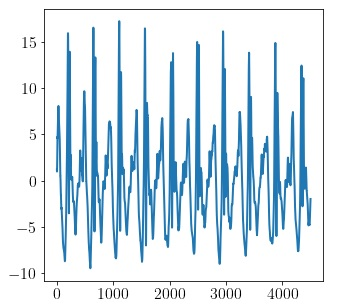
\includegraphics[width=0.5\linewidth]{ts.jpg}}
	    \caption{Исследуемый временной ряд.}
    \end{figure}
    
Разложение временного ряда с помощью метода главных компонент и его восстановление описано в работе [1]. Количество выбранных главных компонент определяет размерность фазового пространства. По соответствующим собственным векторам восстанавливается временной ряд. Анализ ошибки MAPE в зависимости от размерности фазового пространства позволяет определить оптимальную размерность пространства, в котором фазовая траектория не имеет ярковыраженных самопересечений. Процесс сегментирования фазовой траектории в пространстве меньшец размерностти так же описан в [1].
    
    \begin{figure}[ht]
        \subfloat[]{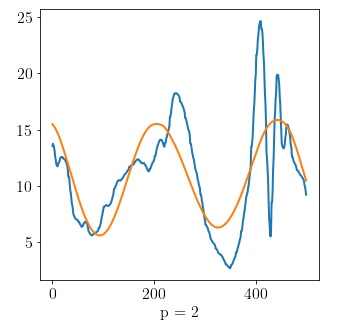
\includegraphics[width=0.32\textwidth]{fig1.jpg}}
        \subfloat[]{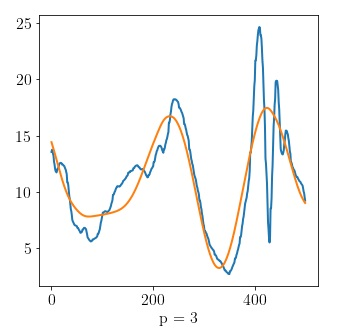
\includegraphics[width=0.32\textwidth]{fig2.jpg}}
        \subfloat[]{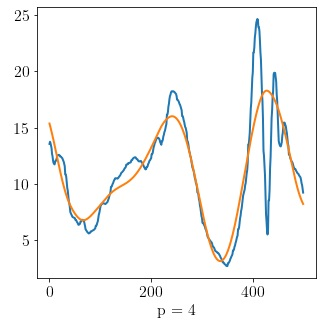
\includegraphics[width=0.32\textwidth]{fig3.jpg}}\\
        \caption{Исходный временной ряд и его разложение для различных размерностей фазового пространства.}
        \label{fg:mod}
    \end{figure}

    
    \begin{figure}[ht]
	    \center{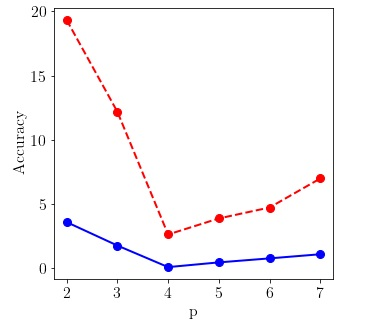
\includegraphics[width=0.5\linewidth]{error.jpg}}
	    \caption{График зависимости точности аппроксимации фазовой траектории от размерности фазового пространства.}
    \end{figure}
    
\newpage

%%%% если имеется doi цитируемого источника, необходимо его указать, см. пример в \bibitem{article}
%%%% DOI публикации, зарегистрированной в системе Crossref, можно получить по адресу http://www.crossref.org/guestquery/

%%%% если имеется doi цитируемого источника, необходимо его указать, см. пример в \bibitem{article}
%%%% DOI публикации, зарегистрированной в системе Crossref, можно получить по адресу http://www.crossref.org/guestquery/.

\end{document} 
